\section{Recovery-Aware Physical Attribution}
\label{sec:narrative-method}

Figure~\ref{fig:joint-architecture} gives the report-level logic. A
history is a proposed cause and trajectory, not just a bus label. The
inference bank predicts the next report under no new event, a new load or
line action, or retained recovery. Its switched predictors come from the
network DAE and oriented PMU terminal map. Statistical filtering handles
uncertain states and residual error. The nonlinear simulator generates the
observations; inference uses local predictors, not a new full simulation
for every hypothesis and report.

\subsection{Construct the Predictor From the Network}

Kirchhoff constraints and complex power connect sources to remote PMUs:
\begin{equation}
 I_{\rm bus}=Y_{\rm bus}V,\quad
 I_{{\rm term},r}=Y_{{\rm term},r}V,\quad S_i=V_i I_{{\rm bus},i}^{*}.
 \label{eq:narrative-electrical}
\end{equation}
Terminal rows retain orientation, line charging and transformer ratios.
A measured terminal current is not a nodal injection. A line opening
changes the branch stamp and therefore the algebraic voltages and measured
currents. A terminal map changes directly only if the switched branch is
itself measured; none of the nine tested line candidates is a measured PMU
terminal. The load operator scales both $P_{\rm set}$ and $Q_{\rm set}$
by $1+a$ with the fixed constant-impedance ZIP fractions, while the line
operator switches the selected branch between active and open modes.

The executed plant has 114 differential states, 78 algebraic variables
and 38 load-input coordinates. Its ten Sauer--Pai machines use AVR Type I
with quadratic ceiling and TGOV1 governors, except the bus-39 machine,
which has no external governor or excitation-control inputs. All 19 load
models use constant-impedance ZIP fractions. With injection sign convention,
\begin{equation}
 P_i=(1+a_i)P_i^0\left|V_i/V_{{\rm set},i}\right|^2,\qquad
 Q_i=(1+a_i)Q_i^0\left|V_i/V_{{\rm set},i}\right|^2.
 \label{eq:implemented-load-law}
\end{equation}
Here $P_i^0<0$ represents consumption; reactive injection can be positive
for a capacitive load. The archived equilibrium and voltage setpoints,
including those at buses 31 and 39, define the executed operating point.

On a regular index-one DAE chart with a fixed angle reference,
\begin{align}
 \delta z&=-g_z^{-1}(g_x\delta x+g_u\delta u),\nonumber\\
 \delta\dot x&=A_q^{\rm red}\delta x+B_q^{\rm red}\delta u,\nonumber\\
 A_q^{\rm red}&=f_x-f_zg_z^{-1}g_x,\quad
 B_q^{\rm red}=f_u-f_zg_z^{-1}g_u.
 \label{eq:narrative-reduction}
\end{align}
For the instantaneous electrical observation map $H_q(x,z,u)$, the
corresponding output operators are
\begin{equation}
 C_q^{\rm red}=H_x-H_zg_z^{-1}g_x,\qquad
 D_q^{\rm red}=H_u-H_zg_z^{-1}g_u.
 \label{eq:electrical-output-reduction}
\end{equation}
They propagate a perturbation at an unmeasured source to the selected
voltage and oriented-current channels. Network connectivity enters through
the branch stamps in $g_q$ and, where applicable, $H_q$; eliminating unmeasured algebraic
variables generally produces dense reduced operators. The graph therefore
constrains the prediction without a learned graph embedding. A changed
terminal operator would also contribute directly through $H_q$; the
tested line modes keep the same terminal map. The implementation discretizes the admitted
switch modes and adds causal phase-history operators for frequency and
ROCOF. The generator estimates phase derivatives with a robust,
magnitude-weighted quadratic fit over 21 reports. The predictor approximates
that operation with a fixed unweighted quadratic fit over the same history;
these operators need not agree when weights change. Inertia, controls and
load law remain those of the fixed plant.

After augmenting instrumental memory, a conditional predictor has the
local form
\begin{align}
 \xi_{k+1}&=A_{\ell,q}\xi_k+b_{\ell,q}+B_{\ell,q}a+w_k,\nonumber\\
 r_k&=C_{\ell,q}\xi_k+d_{\ell,q}+D_{\ell,q}a+v_k.
 \label{eq:implemented-predictor}
\end{align}
Here $r_k$ contains reference-corrected, scaled and instrument-whitened PMU coordinates, $\ell$ is a fixed
network hypothesis, and $\xi_k$ contains physical deviation states, phase
history and predicted measurement-filter memory. Observed colored-instrument
filters whiten measurements; their corresponding predictor memory is
deterministic. Additional latent AR states represent persistent discrepancy,
with preset quiet/load/line/recovery covariance and drift regimes. This
statistical discrepancy model is distinct from the plant equations.
$v_k$ denotes the remaining innovation. A load has scalar severity within
its specified P/Q direction. A line uses a switched operator rather than
a fictitious load-amplitude fit. Equation~\eqref{eq:implemented-predictor} states the generic local model;
the implemented update combines propagation and observation into an
operator on the previous state. The supplement gives that indexing and
the associated transition gain explicitly. States from different equilibria are not
interpreted as an absolute rotor-state mixture.

\subsection{Estimate Context From the Startup Prefix}

Each network hypothesis uses the same 300 startup reports to estimate
operating factors, reference phase and noise scale. Voltage/current
coordinates receive a constant discrepancy correction,
\begin{equation}
 \widehat b_\ell=\overline y_{0:299}-y_\ell^{\rm ref},
 \qquad b_{\ell,k}=\widehat b_\ell\quad(k\ge300).
 \label{eq:continuous-intercept}
\end{equation}
Angular differences respect wrapping and the common reference. Frequency
and ROCOF use empirical prefix centers. The correction remains fixed so it
cannot track a later load step and subtract its signature. This estimates
an observation discrepancy, not the true impedances. Prefix estimates
enter by substitution rather than through a full joint parameter posterior.

\subsection{Compare Unknown-Onset Histories}

The method retains ten seconds of past conditional states. Its frozen birth screen proposes selected onsets at 19 candidate lags,
0--18, within a 20-report candidate window. It does not enumerate every
onset in the 300-report history.
Each history specifies family, asset, onset,
restoration mode and severity. It starts from the stored conditional state
before its proposed onset. That state already contains any ongoing
recovery; an alarm does not reset the predictor to equilibrium.

For a retained load history, conditional Gaussian filtering yields a
residual $e$, severity response $s$ and covariance $S$. Unknown severity
has a truncated-Gaussian distribution inherited from previous reports:
\begin{equation}
 L_{h,k}=\int_l^u \mathcal N(e;sa,S)
             \operatorname{TN}_{[l,u]}(a;\mu,v)\,da.
 \label{eq:narrative-evidence}
\end{equation}
The supplement derives the closed form by completing the square and
works through a numerical example. It also specifies the conditional
state representation $m_h+d_h a$ and its update. The local amplitude
integral is exact for the stated conditional Gaussian model. The complete
bank remains approximate: regime covariances are shared from
nominal-operator Riccati equations, context estimates enter by substitution,
and histories are screened and pruned. At episode closure the augmented
state mixture mean is retained and omitted between-history spread is recorded.
A fully Bayesian posterior over states, context and all histories is not claimed.

The rolling screen proposes histories; it is not another independent
observation. Replaying a suffix replaces its original no-new-event suffix
likelihood. The sequential update therefore counts each report once,
rather than repeatedly accumulating overlapping ten-second windows.

Within each fixed network hypothesis $\ell$, let $\mathcal H_{\ell,k}$
denote its screened non-null histories and
$\mathcal A_{\ell,k}=\mathcal H_{\ell,k}\cup\{0\}$ include the
null history $0$ (no intervention). For each currently admitted candidate
$h$, let $\bar\pi_{\ell,h,k}$ denote its predicted mass before scoring the
current report. For an existing history this prediction applies the
implementation's OFF hazards to survivors and children, generated on demand.
For a proposed birth at report $\tau$, it includes the null-parent mass,
the frozen birth prior, and the replay likelihood ratio
$\exp(\ell^{\rm new}_{\tau:k-1}-\ell^{\rm old}_{\tau:k-1})$ with the
corresponding transition and prior terms. Thus the proposal replaces the
old no-event suffix before the current report is scored; the reports in the
replayed suffix are not counted twice. The supplement gives the corresponding score identity. The report update and within-hypothesis
normalization are
\begin{align}
\widetilde\pi_{\ell,h,k}&=L_{\ell,h,k}\bar\pi_{\ell,h,k},\qquad
\widetilde\pi_{\ell,0,k}=L_{\ell,0,k}\bar\pi_{\ell,0,k},\nonumber\\
\pi_{\ell,h,k}&=\frac{\widetilde\pi_{\ell,h,k}}
 {\sum_{j\in\mathcal A_{\ell,k}}\widetilde\pi_{\ell,j,k}}.
\label{eq:history-mass-update}
\end{align}
This is a normalization scheme for the currently admitted candidates, not
a full Markov transition over all possible histories. After each update, the
screen and beam prune hypotheses and the retained masses are renormalized
jointly with the null. The outer weights $w_{\ell,k}$ are updated from
network-level predictive densities and combine these conditional masses in
$M$ and $\Gamma$; they are not part of the within-bank normalizer. The
resulting masses do not define a calibrated posterior.

\begin{figure*}[t]\centering
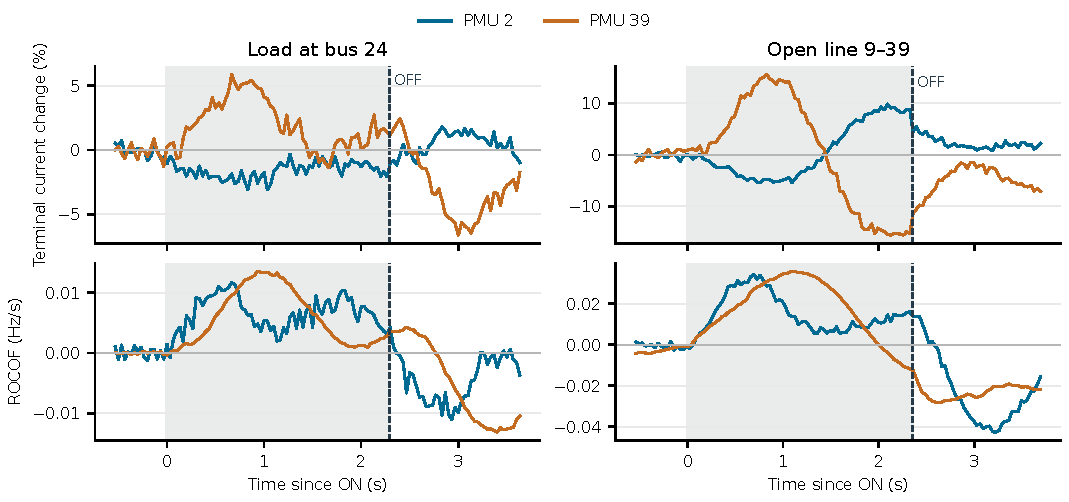
\includegraphics[width=.91\textwidth]{figures/generated/reader_observed_signals.pdf}
\caption{Two interventions from one continuous development record. Current change and ROCOF at PMUs 2 and 39 remain dynamic after physical OFF (dashed line). The gray interval is the true active period, shown only for explanation; inference uses all eight PMUs without event timing. These two PMUs illustrate the traces and were fixed for both panels.}
\label{fig:narrative-signals}\end{figure*}

\subsection{Represent Fixed Network Uncertainty}

The bank contains nominal, global $\pm2\%$, and selected-branch $\pm3\%$
paired R/X hypotheses. Parameters stay constant within a hypothesis. Its
outer weight uses a predictive density formed before the current-report
state update and proposal selection:
\begin{equation}
 w_{\ell,k}=\frac{w_{\ell,k-1}p_\ell(y_k\mid\mathcal F_{k-1},\widehat b_\ell)}
 {\sum_jw_{j,k-1}p_j(y_k\mid\mathcal F_{k-1},\widehat b_j)}.
 \label{eq:continuous-weights}
\end{equation}
Startup-fitting reports are not scored again as independent model-selection
evidence. The mixture covers a finite set of network alternatives rather
than identifying a continuous impedance posterior.

\subsection{Keep Recovery as a Competing Physical Explanation}

Restoring an input or topology at $\kappa$ does not restore the pre-event
state: $x(\kappa^+)=x(\kappa^-)$. On a regular local post-restoration chart,
the difference from a same-context no-new-intervention trajectory obeys
\begin{align}
 \delta x_h(t)&\simeq\Phi_0(t,\kappa)\delta x_h(\kappa),\nonumber\\
 \delta y_h^{\rm net}(t)&\simeq C_0(t)\Phi_0(t,\kappa)\delta x_h(\kappa),
 \quad t>\kappa.
 \label{eq:recovery-response}
\end{align}
Here $y^{\rm net}$ denotes voltage/current coordinates before the instrument map.
Instrumental memory is retained as well. This local interpretation of known
dynamics explains why the reference after OFF is a trajectory, not a zero
residual; it is not a new propagation theorem.

For conditional history mass $\pi_{\ell,h,k}$, define active and
originating-cause masses for an admissible family/source cell $c$:
\begin{align}
 M_{c,k}&=\sum_\ell w_{\ell,k}\sum_{h:c(h)=c}
       \pi_{\ell,h,k}\,\mathbf1\{h\text{ active at }k\},\nonumber\\
 \Gamma_{c,k}&=\sum_\ell w_{\ell,k}\sum_{h:c(h)=c}\pi_{\ell,h,k}.
 \label{eq:active-cause-masses}
\end{align}
A retained history can stop being active while its cause still explains
recovery. Later interventions compete with those histories. The
implementation stores 18 admissible cells, not every family at every bus.
After confirmed episode closure, explicit histories are compressed into
the retained state mean. Cause masses describe the current bank, not a
permanent ledger of all past interventions.

Writing the conditional active mass as $M_{\ell,c,k}$ yields
\begin{align}
 \Delta M_{c,k}&=\sum_\ell w_{\ell,k}
               (M_{\ell,c,k}-M_{\ell,c,k-1})\nonumber\\
 &\quad+\sum_\ell(w_{\ell,k}-w_{\ell,k-1})M_{\ell,c,k-1}.
 \label{eq:continuous-delta}
\end{align}
The terms distinguish within-model evolution from model reweighting.
This accounting identity aids interpretation, without constituting a new
tensor factorization. The masses are approximate attribution weights;
probability calibration and globally optimal filtering are not established.

\subsection{Emit Separate Detection, Diagnosis and Restoration Messages}

The internal observer proposes an alarm after the six-report persistence
rule above the 0.99 active-mass threshold. Public alarm publication additionally requires an
internal pending episode and six reports of qualified active support:
the frozen source screen qualifies load cells, while admitted line cells
qualify through their switched operator. Public OFF requires six reports
above 0.99 for the diagnosed cell's joint cause-and-restoration mass.
The observer also has a separate, more conservative 15-report internal
OFF clock. Diagnosis selects the family with greatest summed cause mass and then
the highest-mass source within that family. It is emitted after six
reports of stable cause support or at the 15-report post-alarm deadline.
The supplement defines the source screen, early line rule and episode
replacement, including how internal messages are propagated publicly. Every message records emission time and
the last report used. A diagnosis can be correct eventually but too late
to precede physical OFF.

The nominal comparator uses the same nominal conditional model with its
own fixed publication path. Comparing nominal and mixture evaluates two
complete configured procedures; it does not isolate the outer network bank
from publication decisions. The admission-rule ablation tests a different publication
decision; it is not a pure recovery-memory ablation.

The supplement records the frozen birth/restoration hazards, severity
prior and integration intervals, restoration-child rules and beam limits,
together with the execution sequence and illustrative calculations.
These details preserve the archived configuration; the compact algorithm
below states the report order and information boundary.

\subsection{Per-Report Algorithm and Computational Boundary}

\noindent\textbf{Algorithm 1: one causal update.}
Input: nominal model, fixed method configuration and PMU reports.
Initialize context, reference, noise and conditional states from the 300
startup reports. Event truth is never an input.
\begin{enumerate}
\item Transform report $k$; predict it from each retained physical or
recovery history. Save each network model's predictive density before
screening or correcting with this report.
\item Screen 19 candidate onset lags (0--18) within the 20-report window. Start each proposed history
from its stored pre-onset state and replay its suffix, replacing the old
suffix likelihood once.
\item Score histories, integrating load severity or using the switched
line operator. Then correct state and severity, update network weights,
and prune by the fixed rules. Retain state and cause through restoration.
\item Aggregate active mass $M$, cause mass $\Gamma$ and $\Delta M$.
Apply the frozen alarm, source and OFF rules; record emission time,
estimated onset and last report used.
\end{enumerate}
The nonlinear simulator constructs observations; this algorithm propagates
local switched predictors. The input grid is 30 reports/s. Causality
concerns report availability; acquisition throughput, computation time
and the electrical history needed for a decision are separate quantities.
Wall-clock real-time operation has not been established.
